%%%%%%%%%%%%%%%%%%%%%%%%%%%%%%%%%%%%%%%%%%%%%%%%%%%%%%%%%%%%%%%%%%%%%%%%%%%%%%%
% intro.tex: Introduction to the thesis
%%%%%%%%%%%%%%%%%%%%%%%%%%%%%%%%%%%%%%%%%%%%%%%%%%%%%%%%%%%%%%%%%%%%%%%%%%%%%%%%
\chapter{Introduction}
\label{intro_chapter}
%%%%%%%%%%%%%%%%%%%%%%%%%%%%%%%%%%%%%%%%%%%%%%%%%%%%%%%%%%%%%%%%%%%%%%%%%%%%%%%%

Kepler's laws of planetary motion, published over a period from 1609 to 1619, describe the motion of planetary orbits as ellipses about a central mass, predicting their orbital period and velocity based on the distance of the semi-major axis \cite{kepler, russell}.
Shown by Isaac Newton in 1687 \cite{newton} to arise directly from his laws of motion and gravitation, Kepler's laws are well understood, extensively tested within our solar system, and, when applied to stellar orbits based on luminous matter in rotating galaxies, highly inconsistent with observation.

The first hint of a problem was found by Jan Oort in 1932, when he measured the velocities of stars in the solar neighborhood. 
Though later found to be inconsistent with modern measurements, Oort observed that the stars he measured were all moving faster than expected based on the visible mass distribution.
Later, Fritz Zwicky measured the velocity of stars in the Coma Cluster and in a 1937 paper \cite{Zwicky} used the virial theorem to predict the total mass of the cluster, finding it to be around two orders of magnitude larger than expected from the cluster luminosity. 
Several other experiments observed similar effects over the following decades, which were generally attributed to light absorption within the galaxies or other systematic errors.

The first measurement of a galaxy rotation curve that agrees with modern observations was made in 1957 by Hendrik van de Hulst using the Dwingeloo 25 meter telescope \cite{deHulst}, which confirmed earlier suspicions that the velocities did not match what was expected using only the luminous matter.
Later, a 1980 survey of 21 spiral galaxies lead by Vera Rubin \cite{RubinSurvey} made precise measurements of the stellar velocity and verified earlier measurements showing unexpectedly high orbital velocities, additionally finding that this excess velocity was present in \textit{all} galaxies surveyed, covering a wide range of luminosities and radii.

Not only did the rotation curves indicate that the mass distribution of the galaxies studied did not match the luminous matter - the increasing velocities to the outermost stars suggests that this excess matter extended some distance beyond the galaxies themselves. 
Basic calculations found that, if Newtonian gravity still held, the excess matter must outweigh the known matter by a significant margin. 
Many theories have been presented to explain these observations, but one of the best motivated theories currently known is that of some unknown "dark matter" particle, which would exist in great abundance throughout the universe and interact very feebly, if at all, with normal matter.
Particulate dark matter is largely favored due to several astronomical observations beyond direct measurement of rotation curves, including measurements of the cosmic microwave background, gravitational lensing, and simulations of galaxy structure formation and baryogenesis in the early universe.

\begin{figure}
   \label{fig:rotCurve}
   \centering
   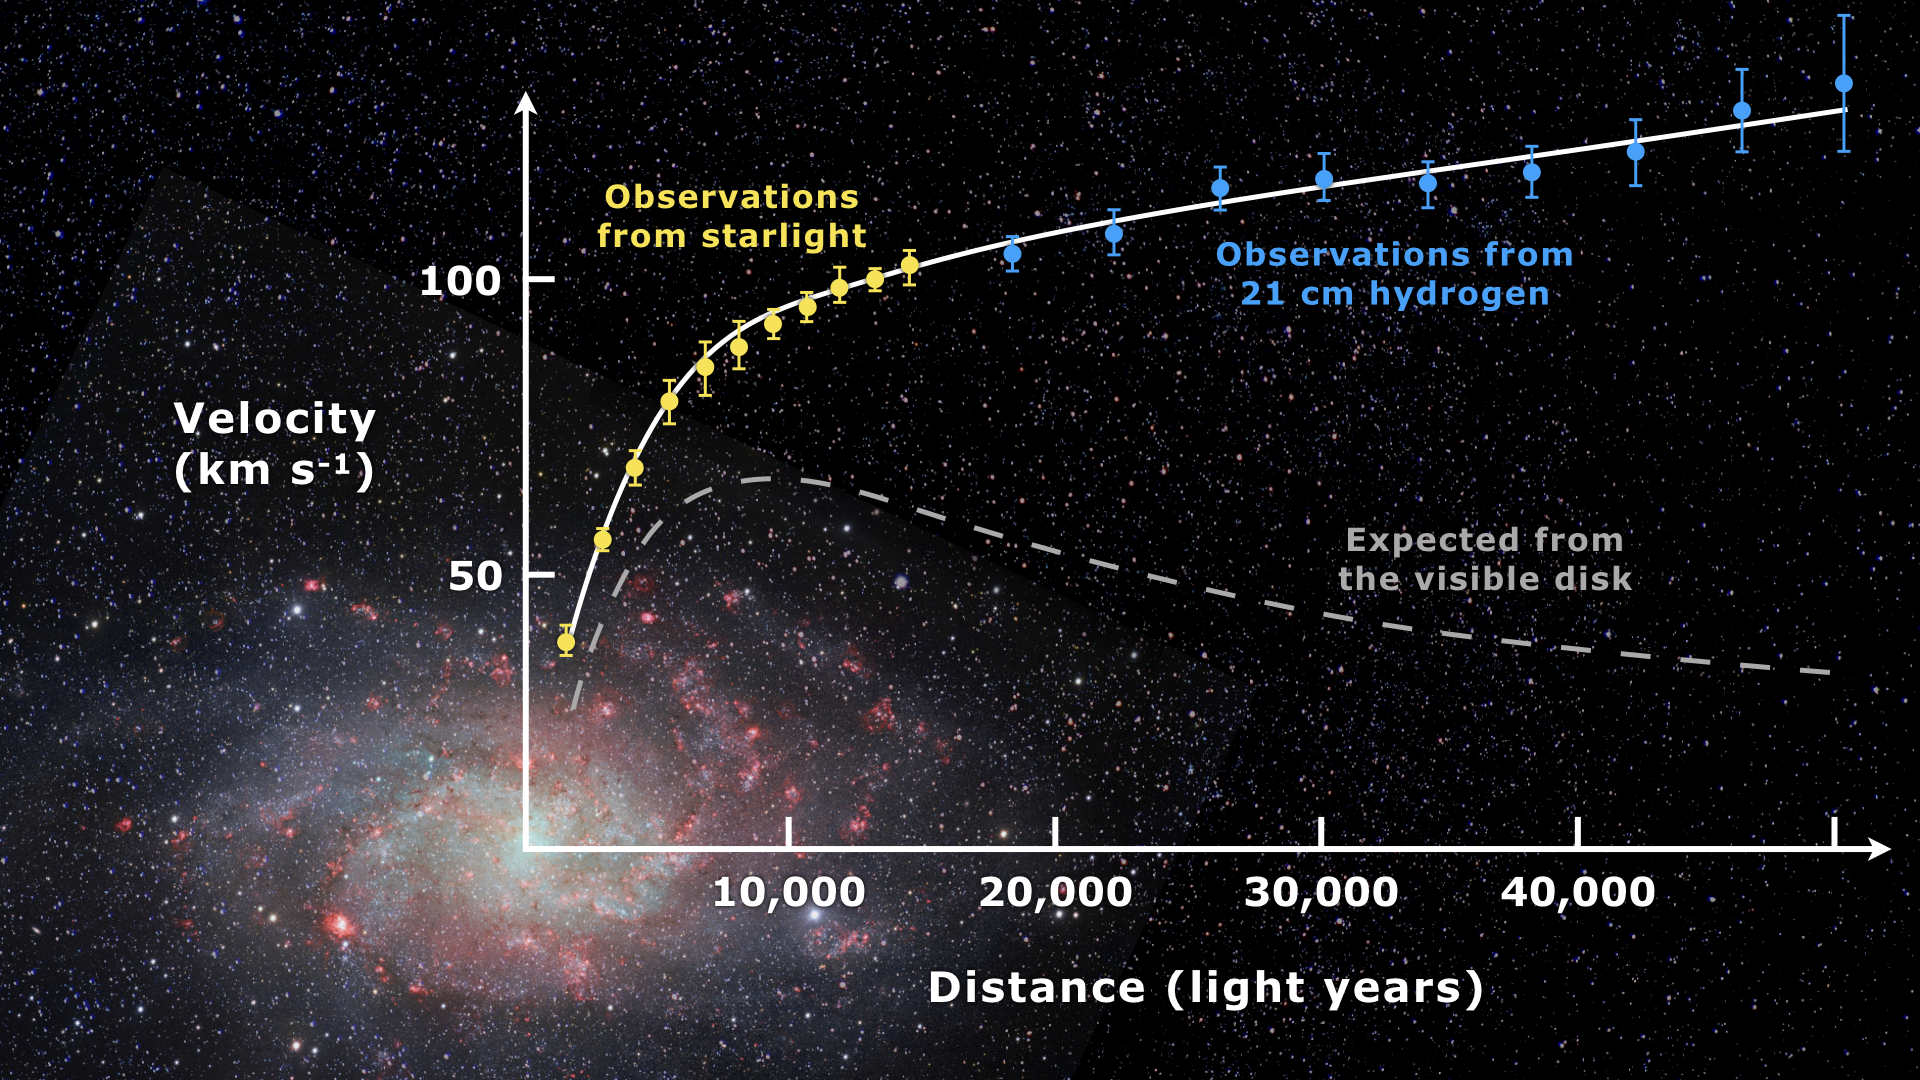
\includegraphics[width=0.6\textwidth]{figures/rotation_curve.png}
   \caption[Rotation curve of Messier 33]{The rotation curve of the spiral galaxy Messier 33, adapted by Mario De Leo from measurements in \cite{Corbelli}. The dashed line shows the expected velocity distribution using only the visible stars, demostrating clear deviation from the observed velocities in both shape and magnitude which could be explained by the presence of a dark matter halo.}
\end{figure}

The strong motivation for a particle explanation of dark matter has lead to an extremely broad scientific program to search for its detection beyond astronomical observations. 
While the mass density and distribution of dark matter is well constrained, almost nothing is currently known about its origins, particle mass, and interactions.
Potential dark matter particle candidates cover an extremely wide range of masses, from \SI{e-22}{\eV}, where the de Broglie wavelength of dark matter becomes too large for the observed galactic structure, to \SI{5e19}{\giga\eV}, where proton interaction with CMB photons would make the universe opaque to high energy photons over large distances.
To help narrow the range of potential signals, several classes of dark matter are defined which have promising features beyond reproducing the correct astronomical observations. 

Among these is light dark matter, where dark matter may interact with standard model particles via mixing with the electromagnetic force. 
This type of mixing would allow dark matter to be produced in the early universe by interactions in the quark-gluon plasma, which would subsequently 'freeze-out', leaving behind the observed relic density seen today. 
Additionally, thermal relic models produce target cross sections for any given dark matter mass as the freeze-out point and corresponding cross section are constrained by the necessary number density to match the known mass density, creating useful experimental goals.
If these mixing terms between dark matter and standard model photons exist, then physics interactions which produce standard model photons could instead very rarely produce 'dark' photons, massive vector bosons with very weak couplings to standard model matter and substantial coupling to stable dark matter particles.

In this thesis, a search for a dark-photon-like signal is performed by looking for 'disappearing' muons in the compact muon solenoid (CMS) experiment. 
As muons pass through materials, they can emit photons through a process known as 'Bremsstrahlung'. 
If Bremsstrahlung were to occur with a dark photon instead of a photon, the emitted \aprime would be kinematically favored to carry most of the incoming muon momentum and would appear invisible to our detector, causing the muon to 'disappear', or have large energy loss without visible energy deposits within the detector.
By measuring the rate that muons disappear within the detector, limits can be set on the frequency of this potential interaction and thus the amplitude of potential mixing between light dark matter and standard model matter.

By looking for new physics interactions between muons and the detector itself, the CMS detector is used as a 'fixed target' experiment rather than the standard collision experiment, where the most relevant physics happens in the initial interaction.
This poses several unique challenges for the analysis.
Muons must be identified with reduced detector information, as the target signal process will modify their behavior and break assumptions used in the standard particle reconstruction algorithms.
Triggers must be identified which keep signal events at reasonable rates.
Rather than simulating the new physics process in an external event generator and importing it into the detector simulation, it must be directly written into the simulation of the detector response, with the ability to calculate the total and differential cross section in a variety of materials over a range of incident muon energies to accurately simulate the interaction for any given muon.

To accomplish this, muons are selected which originate from Z-bosons, which peak strongly in invariant mass near \SI{91}{\giga\eV}, so that one muon can be used to trigger the event and the other can be extrapolated into the detector to search for potential energy loss.
Because the probability of a fixed target interaction occurring is proportional to the amount of material traversed, we focus on muons passing through the CMS hadronic calorimeter, which forms the thickest sensitive part of the detector.
Lastly, signal events are categorized into two regions based on their behaviors in the muon systems, the outermost part of the detector. 
Events with no reconstructed muons nearby are classified as 'complete disappearance', while those with large energy differences between the probe track and the muon chamber track are classified as 'partial disappearance' events.
By using these two categories, the rate of muons undergoing invisible energy loss is determined and then used to set a limit on the potential coupling between standard model photons and potential dark matter mediators.

%%%%%%%%%%%%%%%%%%%%%%%%%%%%%%%%%%%%%%%%%%%%%%%%%%%%%%%%%%%%%%%%%%%%%%%%%%%%%%%%
